\chapter{Analisis Masalah dan Perancangan Solusi}

\section{Analisis \textit{Speech Recognition}}

Ada beberapa permasalahan yang ditemukan pada permasalahan pengenalan ucapan, dan salah satunya dan yang menjadi fokus pada riset ini adalah kesulitan sistem pengenal ucapan dalam mengenali suara pada lingkungan yang bising. Beberapa riset-riset terkait mengenai permasalahan tersebut mencoba untuk menyelesaikannya dengan menambahkan informasi visual pada proses pengenalan suaranya, seperti pada riset \textcite{Chung2017}, \textcite{Chung2016}, dan \textcite{Assael2016}.
\bigskip

Untuk riset-riset yang menggunakan bahasa Indonesia sejauh ini sudah banyak yang menggunakan pendekatan \textit{deep learning} akan tetapi belum ada riset yang menggabungkan fitur akustik dan fitur visual, baik yang menggunakan fitur \textit{handcrafted} dan model akustik berbasis statistik maupun \textit{deep learning}.


\section{Analisis \textit{Lip Reading}}

Riset-riset terkait \textit{lip reading} bahasa Indonesia masih terbilang sedikit jika dibandingkan dengan riset-riset \textit{lip reading} dengan bahasa lain, terutama bahasa Inggris. Riset mengenai \textit{lip reading} yang menggunakan dataset bahasa Indonesia kebanyakan masih belum menggunakan \textit{deep learning}, seperti pada riset \textcite{Achmad2015} yang menggunakan HMM menunjukkan bahwa hasil pengenalan masih belum tergeneralisasi dengan baik karena hasilnya masih berpengaruh pada kondisi bibir pembicara, yang dalam hal ini pembicara wanita dengan bibir yang menggunakan lipstik memiliki koefisien korelasi yang tinggi sedangkan untuk yang bibir berwarna pucat dan bibir yang memiliki kumis di atasnya memiliki koefisien korelasi yang rendah.
\bigskip

Selain riset tersebut, pada saat penulisan, hanya ada satu paper mengenai \textit{lip reading} dalam bahasa Indonesia yang menggunakan pendekatan \textit{deep learning}, yaitu oleh \textcite{Maulana2018}, yang menggunakan \textit{spatiotemporal} CNN untuk menangkap struktur \textit{spatiotemporal} dari video, dan menggunakan \textit{bidirectional} Gated Recurrent Unit (GRU) untuk memodelkan keseluruhan rangkaian frame video dari dua arah, baik dengan urutan frame normal maupun dengan urutan terbalik.


\section{Analisis Model \textit{sequence-to-sequence}}

Salah satu permasalahan yang ditemui dalam penggunaan model \textit{sequence-to-sequence} untuk mentransduksi sebuah rangkaian menjadi rangkaian lain adalah kebanyakan model ini menggunakan RNN atau variannya sehingga prosesnya tidak bisa diparalelisasi karena sifatnya yang rekurens. Oleh sebab itu, proses pelatihan model membutuhkan waktu yang lama hingga model akhirnya konvergen. Pada riset \textcite{Vaswani2017} di usulkan model yang disebut sebagai model transformer, sebuah arsitektur model yang menghindari penggunaan rekurens dan bergantung sepenuhnya pada mekanisme \textit{attention} untuk menggambarkan dependensi global antara masukan dan keluaran. Selain itu model transformer ini memungkinkan dilakukannya paralelisasi sehingga dapat mempercepat proses pelatihan model, dan juga berhasil mengungguli model \textit{encoder-decoder} berbasis RNN dalam mentransduksi rangkaian.

\section{Usulan Solusi}

Berikut adalah rancangan arsitektur penyelesaian permasalahan pengenalan suara dengan menggunakan fitur akustik dan visual pada bahasa Indonesia.

\begin{figure}[h]
    \centering
    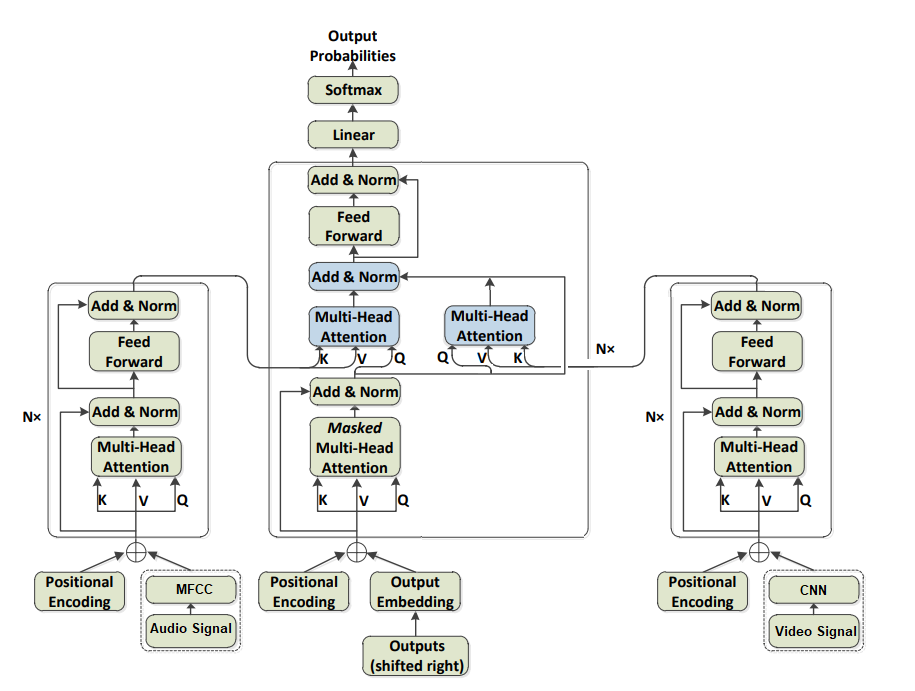
\includegraphics[width=0.8\textwidth]{resources/images/usulan-arsitektur.png}
    \caption{Rancangan Arsitektur.}
    \label{fig:usulan-arsitektur}
\end{figure}

Rangkaian penyelesaiannya adalah sebagai berikut.
\begin{enumerate}
    \item Melakukan perancangan model akustik dengan menggunakan model transformer (Gambar \ref{fig:usulan-arsitektur}) dan melakukan pelatihan model menggunakan dataset dalam bahasa Indonesia. Masukan yang digunakan adalah \textit{raw speech} yang kemudian diekstraksi fiturnya dengan menggunakan MFCC.
    \item Melakukan perancangan model untuk bagian \textit{visual speech recognition} dengan menggunakan model transformer (Gambar \ref{fig:usulan-arsitektur}) dan melakukan pelatihan model menggunakan dataset dalam bahasa Indonesia. Masukan yang digunakan adalah frame video yang direpresentasikan menjadi \textit{fixed-length vector} dengan menggunakan CNN.
    \item Melakukan penggabungan kedua model ASR dan VSR, dan melakukan pelatihan secara bersama-sama.
\end{enumerate}

Metrik pengujian yang digunakan pada saat pengujian adalah \textit{word error rate} (WER). Pengujian dilakukan dengan membandingkan model ASR dengan model \textit{baseline}nya, lalu selanjutnya melakukan perbandingan model VSR dengan model \textit{baseline}nya, lalu terakhir adalah melakukan pengujian terhadap model gabungan ASR dan VSR dan dibandingkan dengan model ASR saja, model VSR saja, dan \textit{baseline} dari model gabungan ASR dan VSR.

\section{Analisis Masalah}
\blindtext

\section{Solusi Umum}
\blindtext

\section{Rancangan Solusi}
\blindtext